\documentclass[a4paper]{article}

%% Language and font encodings
\usepackage[english]{babel}
\usepackage[utf8x]{inputenc}
\usepackage[T1]{fontenc}

%% Sets page size and margins
\usepackage[a4paper,top=3cm,bottom=2cm,left=3cm,right=3cm,marginparwidth=1.75cm]{geometry}

%% Useful packages
\usepackage{amsmath}
\usepackage{graphicx}
\usepackage{subcaption}
\usepackage[colorinlistoftodos]{todonotes}
\usepackage[colorlinks=true, allcolors=blue]{hyperref}

\title{Investigating Existing Blip Glitches using GravitySpy and Q-Transforms}
\author{Melissa Kohl}
\date{\today}

\begin{document}
\maketitle
\graphicspath{ {images/} }

\section{Background} Write in some detail the motivation for your project. It should include background and an overview of the ongoing work in the research group. You should include references. ~\\

The glitches in the strain data from the science and observation runs of the Advanced LIGO detectors decrease the sensitivity of the detectors and obscure gravitational waves \cite{Zevin:2016}. Although some glitches can be identified and eliminated from the strain data during later analysis, astronomical events that give off additional radiation, such as neutron star mergers, need to be recognized immediately so that astronomers can observe the event. As a result, it is imperative to find the sources of the glitches and eliminate them before future observing runs, directly increasing the sensitivity of the detectors while observing \cite{Mukherjee:2010}. 

The current method for classifying glitches and identifying their sources is a machine learning software package called GravitySpy \cite{Zevin:2016}. Unlike previous machine learning techniques used on LIGO data that only compared the waveforms of the glitches \cite{Mukherjee:2010}, GravitySpy's neural network takes in spectrograms from four different time frames to create a multi-layer network that utilizes image classification techniques \cite{Bahaadini:2017}. Since different types of glitches have different durations, the multiple views not only provide complementary data across time frames, but also allow for identification of a broader group of glitches of different durations \cite{Bahaadini:2017}. GravitySpy is therefore great at classifying glitches into known classifications \cite{Zevin:2016}, but the classifications themselves may be too broad, allowing for glitches caused by different sources to be classified into the same type of glitch if the shapes of the glitches are similar in a spectrogram.

Once glitches are classified, GravitySpy is also used to find similar glitches in the hundreds of thousands of auxiliary channels keeping track of the instruments and environments of each detector \cite{Zevin:2016}. Without classification, GravitySpy cannot identify the sources of glitches.


\section{Approach} Discuss the problem you are working on and explain how it fits into the ongoing work. Explain your approach and outline the methods you have been using or expect to use. ~\\

The most frequently-occurring glitches, such as blip glitches, are likely conglomerates of glitches from different sources that happen to create the same general shape in a spectrogram. Unfortunately, the shape of a blip glitch in a spectrogram is uninspiring, with no weird spikes or unique shapes and little to even distinguish one from another. To identify and eliminate these glitches, I must find a different way to distinguish between blip glitches other than a spectrogram. 

One common way to visualize a glitch or other noise in the strain data is a Q-transform, which is a time-to-frequency domain transform related to the Fourier transform. To gain a better understanding of blip glitches and their characteristics, I started by performing Q-transforms on known glitches from the first observing run at the Livingston detector. 


\section{Work} Discuss the work you have done on your project. What progress have you made? ~\\

I wrote a Python script, adapted from the GWpy Q-transform documentation, to plot the Q-transform of about 30 random glitches, all with the same time domain of 0.30 seconds. While manually looking through the images, I found four distinct types of images, as seen in figure \ref{fig:q_transforms} on page \pageref{fig:q_transforms}. I called the four types normal, burst, dot, and stick for their appearances in the Q-transform, but there is still a lot more investigation needed before making the assumption that these are indeed sub-classes.

\section{Challenges and Problems} What are the challenges and problems you have met so far? What challenges and problems do you anticipate moving forward? ~\\

At the beginning, it was difficult to get familiar with GravitySpy due to the limited amount of documentation, but now I feel more comfortable about GravitySpy and other resources. The biggest problem moving forward is figuring out whether any of the normal attributes of a glitch, such as bandwidth, peak frequency, etc, can be used to distinguish between different subclasses of blip glitches. Additionally, actually trying to create an input for a machine learning algorithm to subclassify these glitches will likely be an arduous task.

\pagebreak


\begin{abstract}

In the Advanced LIGO observation runs, detection of gravitational waves is directly dependent on the sensitivity of the detectors. The strain data contain "glitches" that decrease the sensitivity of the detectors and obscure real gravitational waves. The machine learning software package used to classify these glitches and identify their sources, GravitySpy, is successful when the spectrogram of the glitch has a very distinct and unique shape. However, the spectrogram of one of the most common types of glitches, called a "blip," has an underwhelming shape with no distinct characteristics, making it difficult for GravitySpy to identify a source (or possibly multiple sources). This suggests looking at blip glitches in a format other than a spectrogram, such as a Q-transform, to determine if there are sub-classifications of blips that might have identifiable sources. Fortunately, the Q-transforms of a variety of blip glitches, nearly indistinguishable in a spectrogram, reveal possible distinct subclasses.

\end{abstract}

\section{Background}

The glitches in the strain data from the science and observation runs of the Advanced LIGO detectors decrease the sensitivity of the detectors and obscure gravitational waves \cite{Zevin:2016}. Although some glitches can be identified and eliminated from the strain data during later analysis, astronomical events that give off additional radiation, such as neutron star mergers, need to be recognized immediately so that astronomers can observe the event. As a result, it is imperative to find the sources of the glitches and eliminate them before future observing runs, directly increasing the sensitivity of the detectors while observing \cite{Mukherjee:2010}. 

The current method for classifying glitches and identifying their sources is a machine learning software package called GravitySpy \cite{Zevin:2016}. Unlike previous machine learning techniques used on LIGO data that only compared the waveforms of the glitches \cite{Mukherjee:2010}, GravitySpy's neural network takes in spectrograms from four different time frames to create a multi-layer network that utilizes image classification techniques \cite{Bahaadini:2017}. Since different types of glitches have different durations, the multiple views not only provide complementary data across time frames, but also allow for identification of a broader group of glitches of different durations \cite{Bahaadini:2017}. GravitySpy is therefore great at classifying glitches into known classifications \cite{Zevin:2016}, but the classifications themselves may be too broad. The output function in GravitySpy's neural network is \textit{softmax} \cite{Bahaadini:2017}, which essentially just classifies the input glitch into the classification with the highest correlation, regardless of how high that correlation is. The combination of the multiple-view input and the \textit{softmax} output function allow for glitches caused by different sources to be classified into the same type of glitch if the shapes of the glitches are similar. In the next section, I introduce an example of two different spectrogram shapes (which most likely have different sources) getting grouped into the same classification. 

The most frequently-occurring glitches, such as blip glitches, are likely conglomerates of glitches from different sources that happen to create the same general shape in a spectrogram. Unfortunately, the shape of a blip glitch in a spectrogram is uninspiring, with no weird spikes or unique shapes and little to even distinguish one from another. To sub-classify these blip glitches, we need a different analysis technique that might reveal hidden characteristics. 

Once glitches are classified, GravitySpy is also used to find similar glitches in the hundreds of thousands of auxiliary channels keeping track of the instruments and environments of each detector \cite{Zevin:2016}. Without sub-classification, GravitySpy cannot identify the sources of blip glitches. 

\section{Investigation of Blip Glitches}

One common way to visualize a glitch or other noise in the strain data is a Q-transform, which is a time-to-frequency domain transform related to the Fourier transform. To gain a better understanding of blip glitches and their characteristics, I started by performing Q-transforms on known glitches from the first observing run at the Livingston detector. I wrote a Python script, adapted from the GWpy Q-transform documentation, to plot the Q-transform of about 30 random glitches, all with the same time domain of 0.30 seconds. While manually looking through the images, I found four distinct types of images, as seen in figure \ref{fig:q_transforms} on page \pageref{fig:q_transforms}. I called the four types normal, burst, dot, and stick for their appearances in the Q-transform, but there was a lot more investigation needed before making the assumption that these were indeed sub-classes.

\begin{figure}
	\centering
	\begin{subfigure}{.49\textwidth}
		\centering
		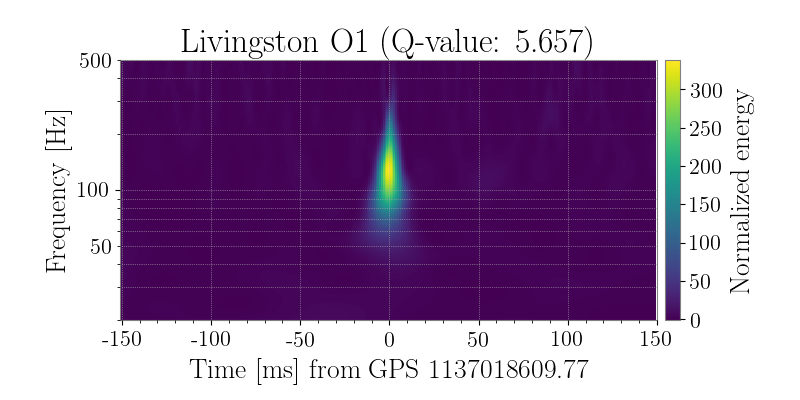
\includegraphics[width=1\linewidth]{normal_blip}
		\caption{Normal blip Q-transform}
		\label{fig:normal}
	\end{subfigure}
	\begin{subfigure}{.49\textwidth}
		\centering
		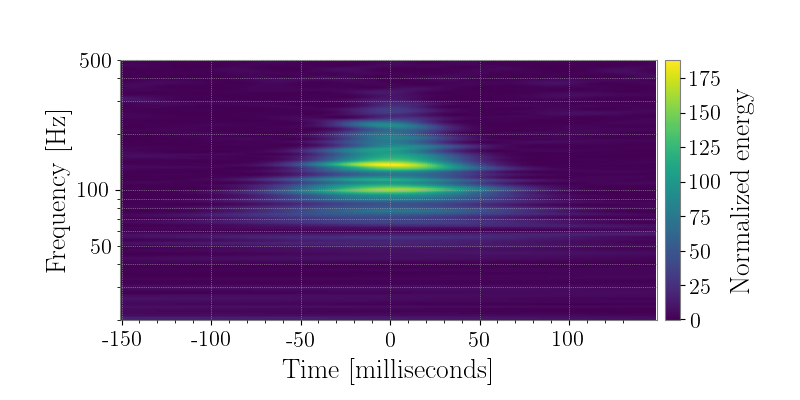
\includegraphics[width=1\linewidth]{burst_blip}
		\caption{Burst blip Q-transform}
		\label{fig:burst}
	\end{subfigure}
	\begin{subfigure}{.49\textwidth}
		\centering
		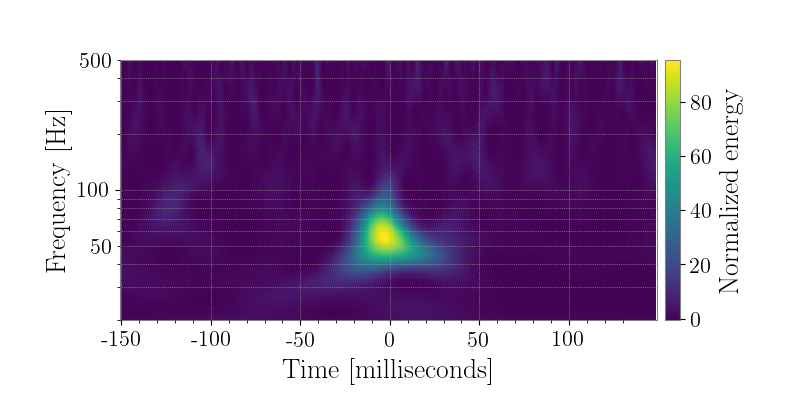
\includegraphics[width=1\linewidth]{dot_blip}
		\caption{Dot blip Q-transform}
		\label{fig:dot}
	\end{subfigure}
	\begin{subfigure}{.49\textwidth}
		\centering
		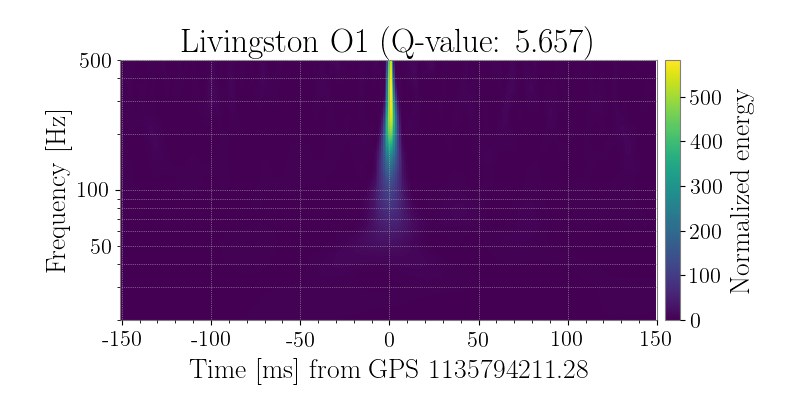
\includegraphics[width=1\linewidth]{stick_blip}
		\caption{Stick blip Q-transform}
		\label{fig:stick}
	\end{subfigure}
	\caption{Four different types of blip glitches in Q-transforms.}
	\label{fig:q_transforms}
\end{figure}

After discovering these differing forms in the Q-transforms and plotting about 100 more Q-transforms, I looked at the spectrograms of a specific glitch of each of the four possible subclassifications to determine the legitimacy of my assumptions, the results of which are in figure \ref{fig:comparison} on page \pageref{fig:comparison}. The most striking difference between the spectrograms and the Q-transforms is from the burst blip. The spectrograms from the normal blip and the burst blip, figures \ref{fig:normal_s} and \ref{fig:burst_s}, appear to be almost exactly the same, but while the normal blip's Q-transform (figure \ref{fig:normal_q}) has the same shape as its spectrogram, hence the name "normal," the burst blip's Q-transform (figure \ref{fig:burst_s}) "bursts" outward with distinct horizontal lines. The burst blip therefore has a good chance of being a true sub-classification of blip glitches. 

The dot blip also has a chance of being a legitimate sub-classification, as its Q-transform (figure \ref{fig:dot_q}) has a distinct round shape at a relatively low frequency compared to the other blips. Unlike the burst, however, the spectrogram of the dot blip (figure \ref{fig:dot_s}) is easily distinguishable from the others, with a much smaller frequency range and an almost triangle-like shape. Since it can be identified on a spectrogram, it is possible that it could be classified apart from other blip glitches by GravitySpy, but it is worth investigating possible attributes of dot blips, such as lower frequency and longer duration compared to other blips..

The stick blip also seems to be different than a normal blip. Its spectrogram (figure \ref{fig:stick_s}) is only slightly skinnier than that of a normal blip, with a slightly longer tail. However, the Q-transform (figure \ref{fig:stick_q}) reveals that a stick blip is at a significantly higher frequency than a normal blip. In this sense, with a higher frequency and shorter duration, stick blips seem to be very separate from dot blips.


\begin{figure}
	\centering
	\begin{subfigure}[t]{.7\textwidth}
		\centering
		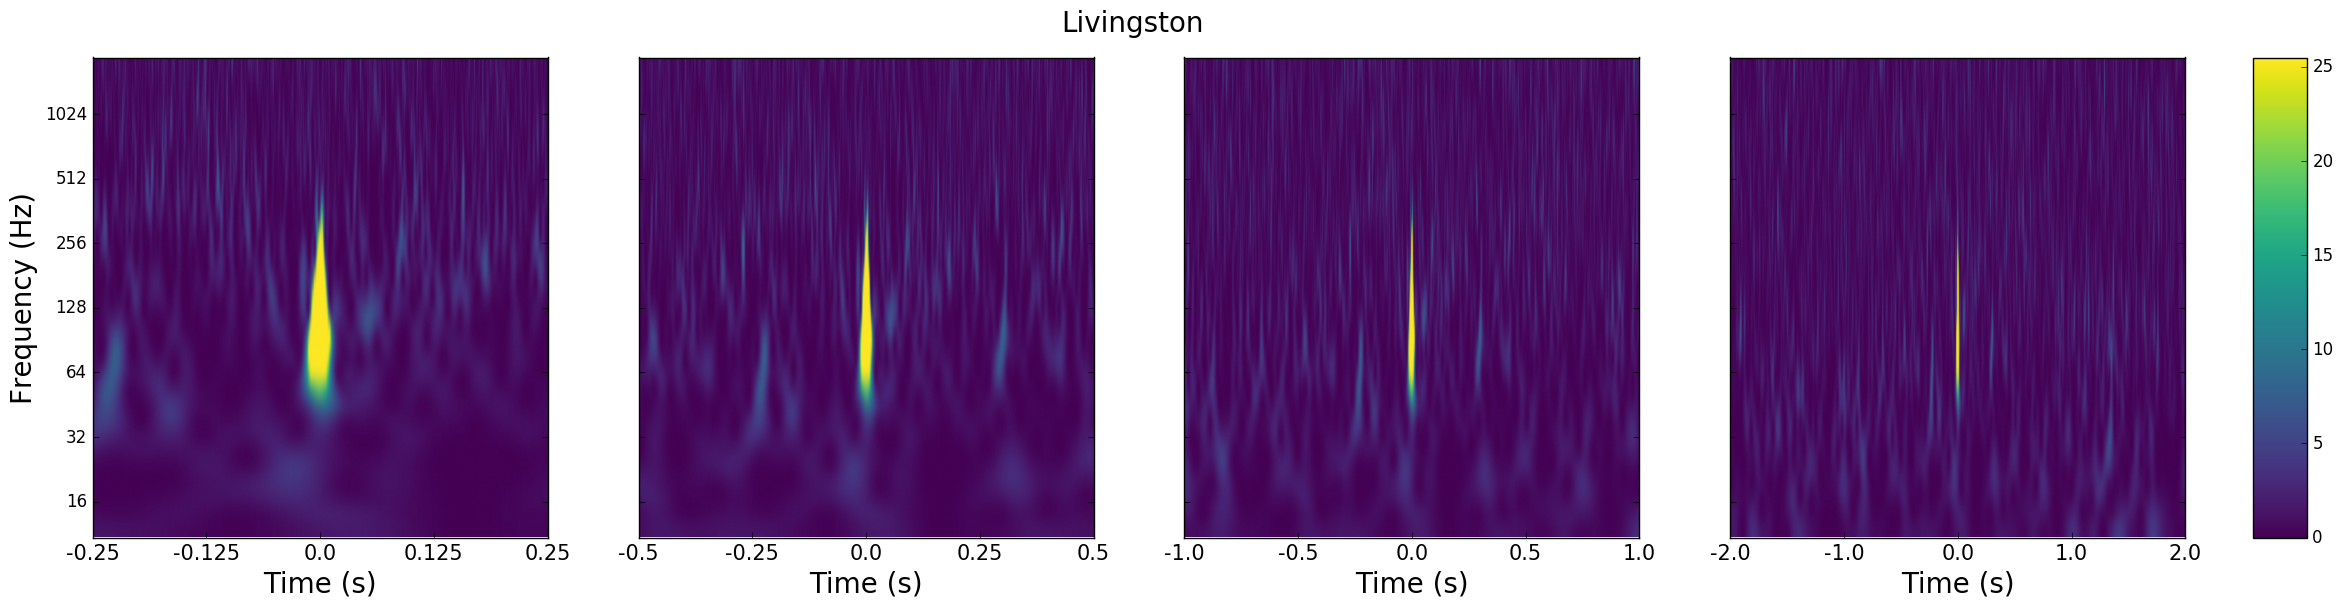
\includegraphics[width=.9\linewidth]{normal_blip_spect}
		\caption{Normal blip spectrograms}
		\label{fig:normal_s}
	\end{subfigure}
	\begin{subfigure}[t]{.29\textwidth}
		\centering
		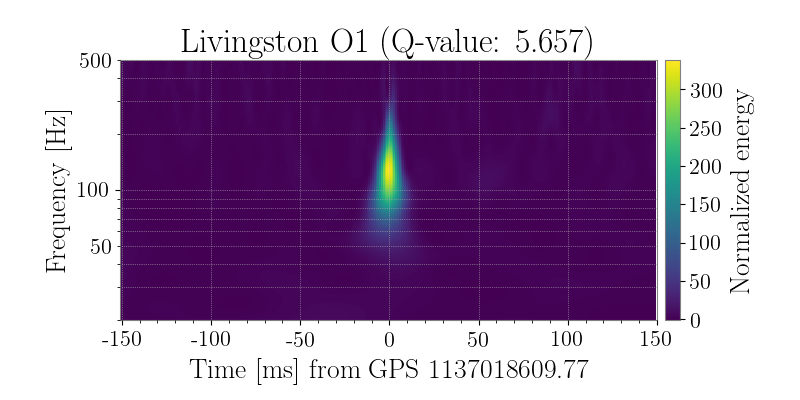
\includegraphics[width=1.1\linewidth]{normal_blip}
		\caption{Normal blip Q-transform}
		\label{fig:normal_q}
	\end{subfigure}
	\begin{subfigure}[t]{.7\textwidth}
		\centering
		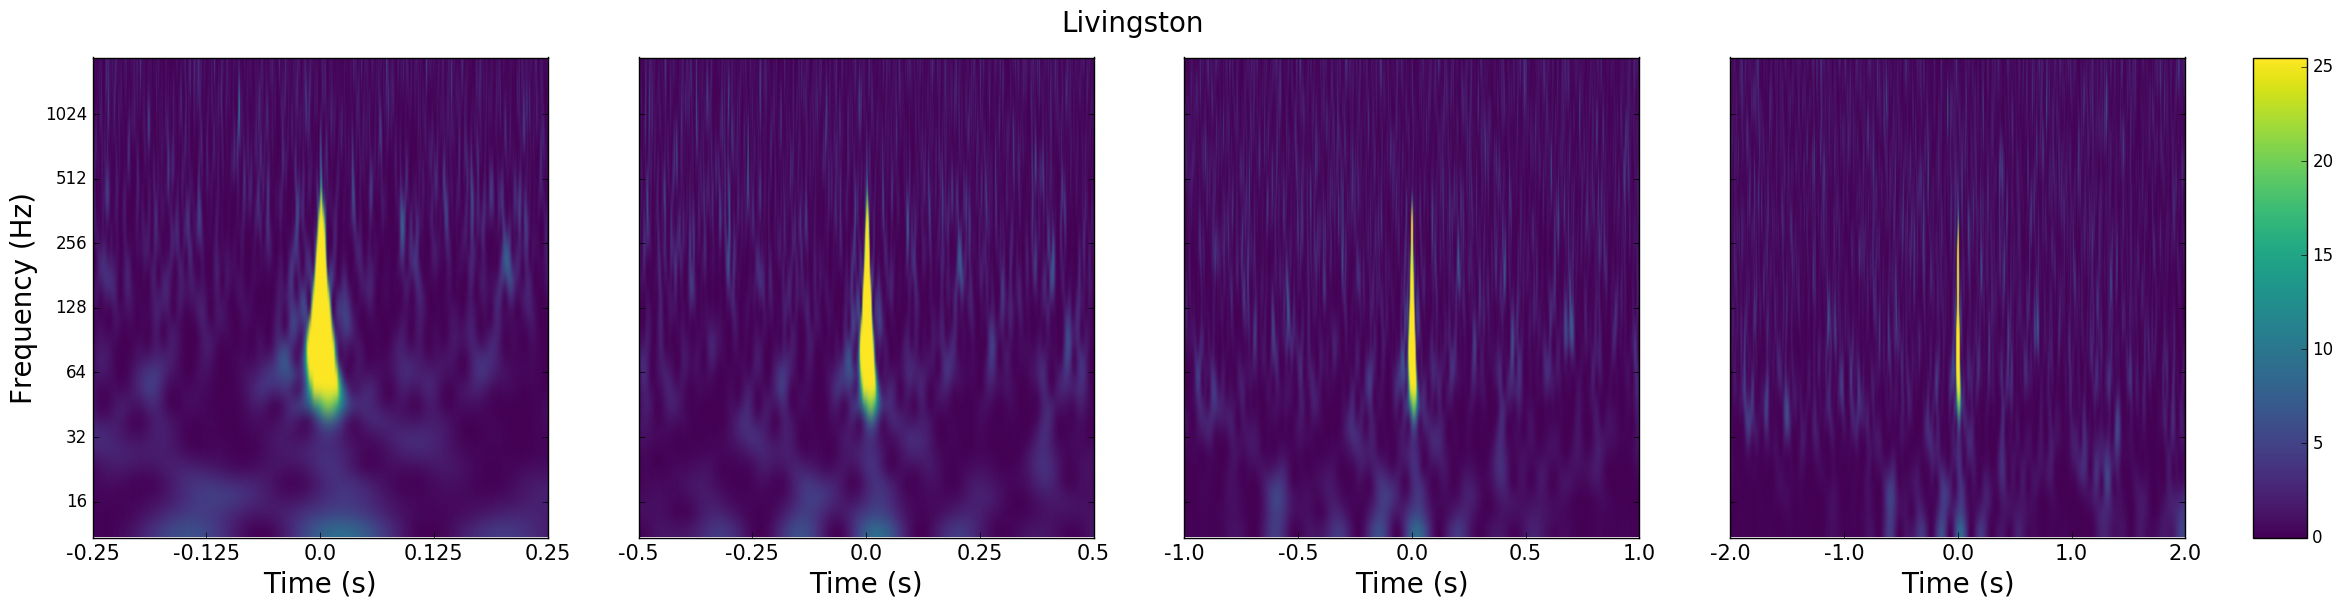
\includegraphics[width=.9\linewidth]{burst_blip_spect}
		\caption{Burst blip spectrograms}
		\label{fig:burst_s}
	\end{subfigure}
	\begin{subfigure}[t]{.29\textwidth}
		\centering
		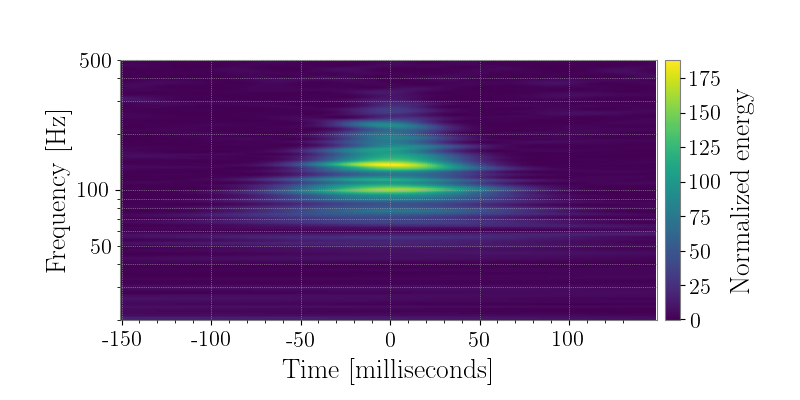
\includegraphics[width=1.1\linewidth]{burst_blip}
		\caption{Burst blip Q-transform}
		\label{fig:burst_q}
	\end{subfigure}
	\begin{subfigure}[t]{.7\textwidth}
		\centering
		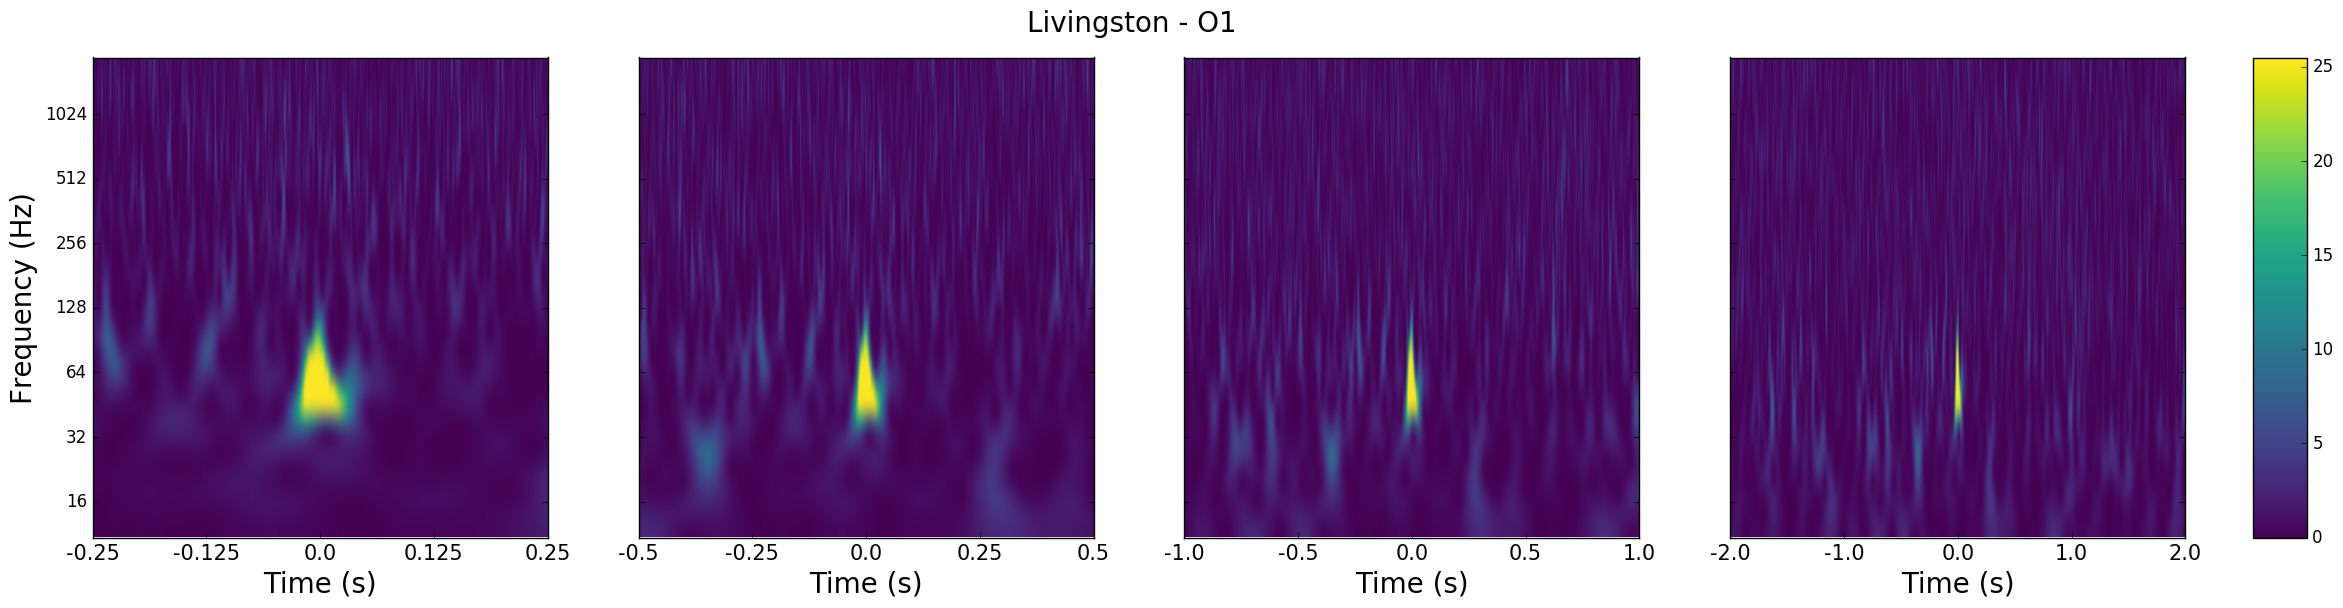
\includegraphics[width=.9\linewidth]{dot_blip_spect}
		\caption{Dot blip spectrograms}
		\label{fig:dot_s}
	\end{subfigure}
	\begin{subfigure}[t]{.29\textwidth}
		\centering
		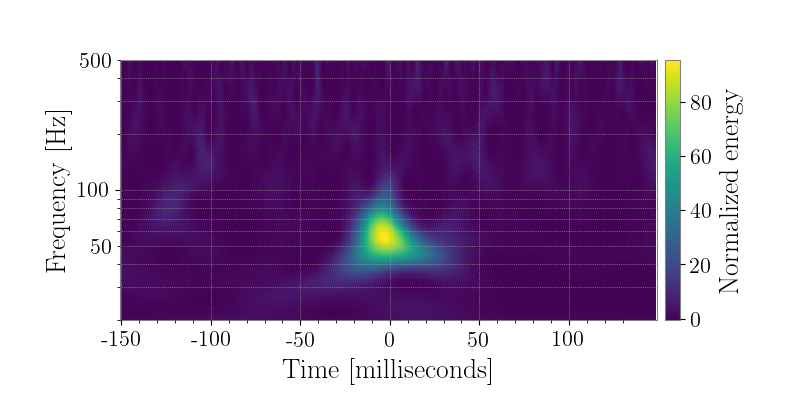
\includegraphics[width=1.1\linewidth]{dot_blip}
		\caption{Dot blip Q-transform}
		\label{fig:dot_q}
	\end{subfigure}
	\begin{subfigure}[t]{.7\textwidth}
		\centering
		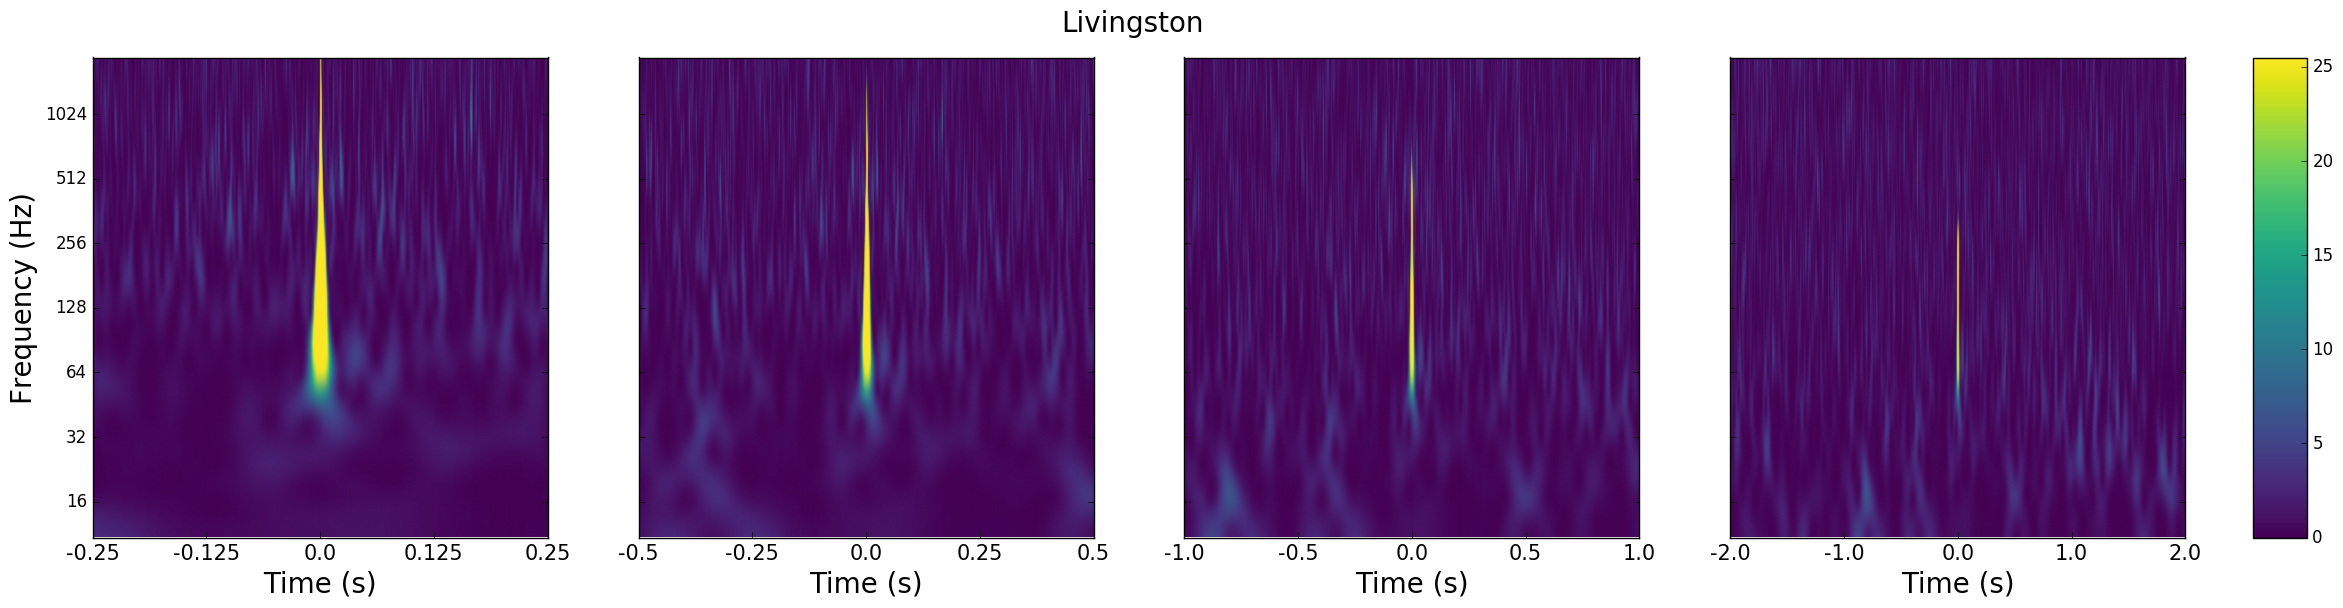
\includegraphics[width=.9\linewidth]{stick_blip_spect}
		\caption{Stick blip spectrograms}
		\label{fig:stick_s}
	\end{subfigure}
	\begin{subfigure}[t]{.29\textwidth}
		\centering
		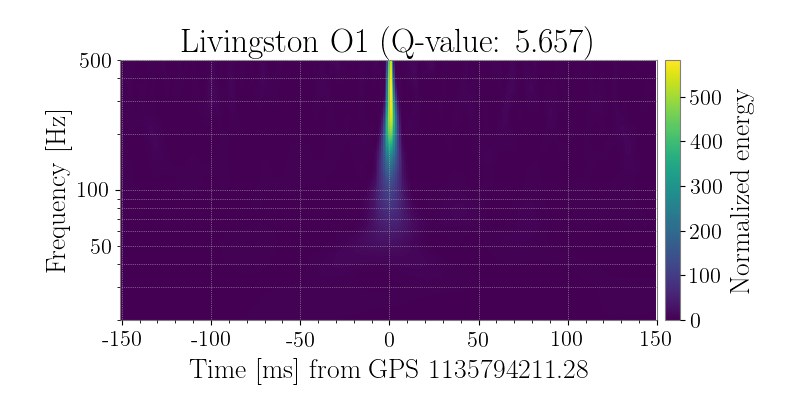
\includegraphics[width=1.1\linewidth]{stick_blip}
		\caption{Stick blip Q-transform}
		\label{fig:stick_q}
	\end{subfigure}
	\caption{A comparison between spectrograms of four different blip glitches on the left and the corresponding Q-transform of the same blip glitches on the right. The top row is a normal blip, the second row is a burst blip, the third a dot blip, and a stick blip on the bottom. Although the spectrograms of the different blips are distinguishable from one another, the Q-transform reveals that these blip glitches are fundamentally different.}
	\label{fig:comparison}
\end{figure}

\section{Determining Distinguishable Characteristics of Possible Sub-Classifications of Blip Glitches}

The first step I took in finding specific attributes to subclassify the blip glitches was sorting glitches by frequency, inspired by the apparent difference between dot blips and stick blips. First looking at blips with an SNR below 12, I modified my Python script to separate the Q-transforms into three peak-frequency bins: lower than 100 Hz, 100-200 Hz, and higher than 200 Hz. 

At low peak frequency, there were no stick blips and a few bursts, but mostly dots and normals. At mid peak frequency, there was a mix of all of the types but still no sticks. At high frequency, there were sticks and a few bursts. So, my assumption that stick blips occur at higher frequency than the rest still holds, but the dot blips couldn't be separated from normal blips based just on frequency. Additionally, the burst blips remain elusive, with a handful in each frequency range.

In an attempt to isolate the burst blips, I looked at blip glitches with a high duration and a low duration. Unfortunately, there were burst blips with high duration and low duration. I then tried the combination of a high duration and low SNR, but again there was no distinction for the burst glitches. 


\bibliography{references}
\bibliographystyle{ieeetr}

\end{document}












